\documentclass[11pt, oneside]{article}   	% use "amsart" instead of "article" for AMSLaTeX format
\usepackage{geometry}                		% See geometry.pdf to learn the layout options. There are lots.
\geometry{letterpaper}                   		% ... or a4paper or a5paper or ... 
%\geometry{landscape}                		% Activate for for rotated page geometry
%\usepackage[parfill]{parskip}    		% Activate to begin paragraphs with an empty line rather than an indent
\usepackage{graphicx}				% Use pdf, png, jpg, or eps� with pdflatex; use eps in DVI mode
								% TeX will automatically convert eps --> pdf in pdflatex		
\usepackage{amssymb}
\usepackage{amsmath}
\usepackage{parskip}

\title{Rotation of coordinates}
%\author{The Author}
%\section{}
% \subsection*{R code}
\date{}							% Activate to display a given date or no date

\graphicspath{{/Users/telliott_admin/Dropbox/Tex/png/}}

% \begin{lstlisting}  \end{lstlisting}
% \begin{center} 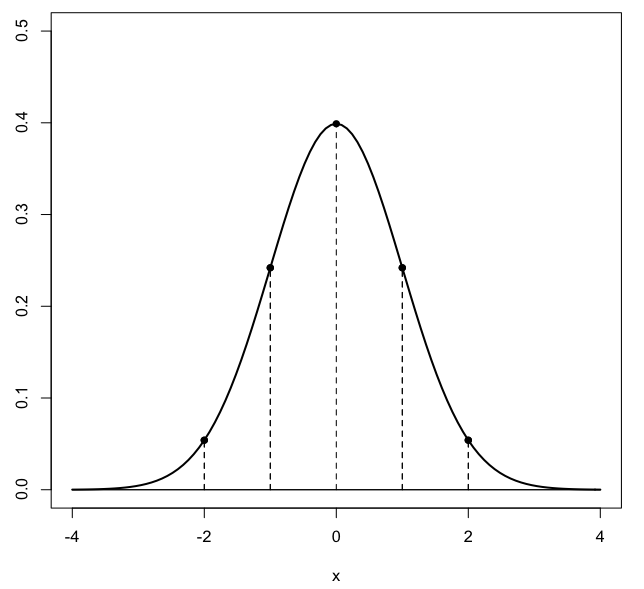
\includegraphics [scale=0.4] {gauss3.png} \end{center}
% \begin{bmatrix} a  &  b \\ c  &  d \end{bmatrix}
% \bigg |_

\begin{document}
\maketitle
\noindent
\Large

I wanted to work on a derivation of the rotation of coordinates formulas.  I've done it before in different ways, but I always have difficulties remembering those proofs.  So here we will just fool around with the algebra a bit.

\begin{center} 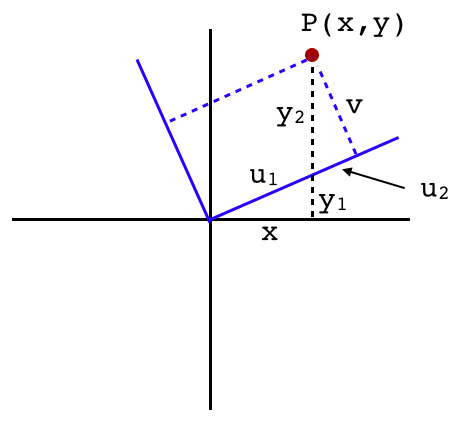
\includegraphics [scale=0.5] {rot1.png} \end{center}

The setup is the usual one.  We have a point $P=(x,y)$ and we want to express the same point in terms of rotated coordinate axes.  This means that we need to find the distances $u$ and $v$ that are the projections of the point onto the new axes.  In the diagram, I express some distances in terms of two components:  $y = y_1 + y_2$ and $u = u_1 + u_2$.

The angle isn't marked explicitly, but let's call it $\theta$.  We can write immediately that
\[ x = u_1 \cos \theta \]
\[ y_1 = u_1 \sin \theta \]

Notice also that the second triangle with labeled sides is similar to the first.  So we can also write
\[ u_2 = y_2 \sin \theta \]
\[ v = y_2 \cos \theta \]

Now we just play with the equations.  We want a function giving $u$
\subsection*{\LARGE{$u = f(x,y,\theta)$}}
Start with
\[ u = u_1 + u_2 \]
We have two equations involving $u_1$.  Multiply the first by $\cos \theta$
\[ x \cos \theta = u_1 \cos^2 \theta \]
Multiply the second one by $\sin \theta$
\[ y_1 \sin \theta = u_1 \sin^2 \theta \]
If we add and then factor out $\cos^2 \theta + \sin^2 \theta = 1$ we obtain:
\[ u_1 = x \cos \theta + y_1 \sin \theta \]
We have that $u_2 = y_2 \sin \theta$ so 
\[ u = u_1 + u_2 \]
\[ u = x \cos \theta + y_1 \sin \theta + y_2 \sin \theta \]
Factor out $y_1 + y_2 = y$
\[ u = x \cos \theta + y \sin \theta \]

\subsection*{\LARGE{$v = f(x,y,\theta)$}}
\[ v = y_2 \cos \theta \]
\[ v = (y - y_1) \cos \theta \]
\[ v = y \cos \theta - y_1 \cos \theta \]

Go back to
\[ x = u_1 \cos \theta \]
\[ y_1 = u_1 \sin \theta \]
\[ y_1 = \frac{x}{\cos \theta} \sin \theta \]

So
\[ v = y \cos \theta - y_1 \cos \theta \]
\[ v = y \cos \theta - \frac{x}{\cos \theta} \sin \theta \cos \theta \]
\[ v = y \cos \theta - x \sin \theta \]

We can use the same equations to get expressions for $x$ and $y$:

\subsection*{\LARGE{$x = f(u,v,\theta)$}}
\[ u = u_1 + u_2 \]
\[ u = \frac{x}{\cos \theta} + y_2 \sin \theta \]
\[ u = \frac{x}{\cos \theta} + \frac{v}{\cos \theta}  \sin \theta \]

We multiply by $\cos \theta$:
\[ u \cos \theta = x + v \sin \theta \]
\[ x = u \cos \theta - v \sin \theta \]

and we have an expression for $x$ in terms of $u$ and $v$ and $\theta$.

\subsection*{\LARGE{$y = f(u,v,\theta)$}}
\[ y = y_1 + y_2 \]
\[ y = u_1 \sin \theta \ + \dots \]

Go back to the two equations involving $y_2$
\[ u_2 = y_2 \sin \theta \]
\[ v = y_2 \cos \theta \]

multiply by either $\sin \theta$ or $\cos \theta$ to obtain:
\[  u_2 \sin \theta = y_2 \sin^2 \theta \]
\[ v \cos \theta = y_2 \cos^2 \theta \]
Add
\[ u_2 \sin \theta + v \cos \theta = y_2 (\sin^2 \theta + \cos^2 \theta) = y_2 \]

Hence 
\[ y = u_1 \sin \theta + y_2 \]
\[ y = u_1 \sin \theta + u_2 \sin \theta + v \cos \theta  \]
\[ y = u \sin \theta + v \cos \theta \]

And we have an expression for $y$ in terms of $u$ and $v$ and $\theta$.

Notice the difference rotating from $xy$ to $uv$
\[ u = x \cos \theta + y \sin \theta \]
\[ v = - x \sin \theta + y \cos \theta \]

while rotating from $uv$ to $xy$
\[ x = u \cos \theta - v \sin \theta \]
\[ y = u \sin \theta + v \cos \theta \]

The difference is a switch from minus to plus and plus to minus on the $\sin \theta$ term.  And the reason is simple, think of the latter rotation as being through the angle $-\theta$, then 
\[ \sin (- \theta) = - \sin \theta \]
\[ \cos (- \theta) = \cos \theta \]

So in comparing rotations by angle $\theta$ in the counter-clockwise and clockwise directions, the difference is just a change in sign for the sine term.

We said the difference rotating from $xy$ to $uv$
\[ u = x \cos \theta + y \sin \theta \]
\[ v = - x \sin \theta + y \cos \theta \]

As a check on our work, consider rotation by $90$ degrees, $\theta = \pi/2$.  We have $\cos \theta = 0$ and $\sin \theta = 1$, so
\[ u = y \]
\[ v = -x \]

which is indeed a counter-clockwise rotation, matching the direction of rotation of the $x,y$-axes to $u,v$ in our diagram.


\end{document}  